\documentclass[a4paper,11pt]{article}

\usepackage{siunitx}
\usepackage[margin=2.2cm]{geometry}
\usepackage{tikz}
\usepackage{url}
\usetikzlibrary{
  arrows.meta,
  calc,
  decorations.pathreplacing,
  patterns,
  positioning
}

\begin{document}
Draft: A Adelmann \today
\section{Beam parameters and first ChDR simulation case}

Let us fix the beam parameters as follows, assuming \SI{60}{MeV} means kinetic energy and \SI{3}{mm} means the longitudinal rms size, denoted $\sigma_x$ because the beam travels along the $x$ axis in the figure:

\[
  E_{\rm kin}=\SI{60}{MeV},\qquad Q=\SI{5}{nC},\qquad
  \sigma_x=\SI{3}{mm}.
\]

The corresponding total energy, relativistic factor and speed are

\[
  E_{\rm tot}=\SI{60.511}{MeV},\qquad
  \gamma=1+\frac{60}{0.510999}=118.417,
  \qquad \beta=\sqrt{1-\gamma^{-2}}=0.99996434.
\]

The bunch duration is $\sigma_t=\sigma_x/c=\SI{10.0}{ps}$.  A Gaussian bunch therefore has an rms-to-FWHM duration of about \SI{23.6}{ps}, and its peak current is

\[
  I_{\rm peak}=\frac{Q}{\sqrt{2\pi}\,\sigma_t}
  \simeq \SI{199}{A}.
\]

The charge corresponds to

\[
  N_e=\frac{Q}{e}=3.12075\times10^{10}\ \text{electrons},
\]

and the bunch kinetic energy is approximately \SI{0.30}{J}.

The current FEL job-file parser does not interpret \texttt{charge} and \texttt{mass} directly as SI coulombs and kilograms.  It converts the numerical entries from electron-charge and electron-mass units into the internal normalized units used by the solver.  Therefore, for a total charge of \SI{5}{nC}, the corresponding entries are

\begin{verbatim}
"charge": 3.1207545e10,
"mass": 3.1207545e10,
"gamma": 118.417071,
"sigma-position": [sigma_x_um, sigma_y_um, 3000.0]
\end{verbatim}

The value \SI{3}{mm} is $3000\,\si{\micro\metre}$.  For the laboratory-frame ChDR model, the computational domain along the beam should cover at least $6$--$10\,\sigma_x$, or roughly \SIrange{18}{30}{mm}, before adding vacuum margins and the dielectric radiator.  

For a Gaussian bunch the longitudinal form factor is

\[
  |F(\omega)|^2=\exp\!\left[-\left(\frac{2\pi\sigma_x}{\lambda}\right)^2\right].
\]

Thus the coherent spectrum is strongest at wavelengths of order $2\pi\sigma_x\simeq\SI{18.8}{mm}$, corresponding to about \SI{15.9}{GHz}.  Coherent visible emission is strongly suppressed for this bunch length; a visible camera signal would require an incoherent single-electron treatment or optical-scale microbunching.  For coherent emission at fixed bunch shape, the radiated power scales approximately as $Q^2$.

The figure below is a schematic laboratory-frame setup.  The dielectric value $\epsilon_r=2.13$ is illustrative, corresponding to $n=\sqrt{2.13}$ and $\theta_{\rm Ch}\simeq46.7^\circ$ at this beam energy.  The impact parameter $a$, transverse beam sizes and radiator dimensions remain geometry parameters for the simulation.

\section{Geometry choice and proof-of-concept scope}

There is no fundamental obstacle to a proof-of-concept simulation.  For $\epsilon_r=2.13$, the value near $47^\circ$ is approximately the internal Cherenkov emission angle,

\[
  \cos\theta_{\rm Ch}=\frac{1}{\beta n},
  \qquad n=\sqrt{\epsilon_r}.
\]

The dielectric surface itself does not have to be tilted by this angle.  A flat dielectric slab parallel to the beam is sufficient to test radiation generation, dependence on the impact parameter $a$, spectrum, polarization and the internal Cherenkov angle.  It does not reproduce the final out-coupling through the prism or the exact camera signal.

\subsection{Limitations to be tackled by the MSc Thesis of D Rosser}
The present FEL mini-app has several limitations for this problem.  
\begin{enumerate}
\item Its field solver assumes vacuum and does not yet support a spatially varying $\epsilon_r(\mathbf r)$, so a dielectric interface has to be added.  An oblique interface on a Cartesian grid also produces staircasing and spurious scattering; an axis-aligned slab is therefore the cleaner first test.  A tilted prism can later be represented with a material mask and subcell averaging or a conformal interface treatment.

\item The FEL implementation uses a Lorentz-boosted frame and treats $z$ as the longitudinal direction.  A stationary radiator requires a laboratory-frame calculation.  The $z$ axis in this figure is consequently a drawing convention unless the code is also rotated or refactored.  

\item Second-order Mur boundaries may reflect oblique waves and dielectric-interface radiation; they are acceptable for an initial test, while PML boundaries are preferable for quantitative power \url{https://arxiv.org/abs/1105.5625}.
\end{enumerate}


\subsection{Experimental Considerations}
\begin{enumerate}
\item With $\sigma_z=\SI{3}{mm}$, coherent radiation is concentrated mainly around \SI{16}{GHz}, so centimetre-scale domains are appropriate.  

\item A visible-camera prediction would require an incoherent single-electron treatment or optical-scale bunching.  

\end{enumerate}

Parameter space for the first POC is therefore a straight \SI{60}{MeV}, \SI{5}{nC} beam passing parallel to a flat $\epsilon_r=2.13$ slab, with the gap $a$ varied.  We can validate the spectrum, polarization and internal $46.7^\circ$ radiation angle before implementing the tilted prism and optical extraction.


\begin{figure}[!t]
  \centering

% Schematic x--y view of a Cherenkov-diffraction-radiation setup.
% The drawing is intentionally schematic; a, sigma_x and the
% radiator dimensions are left as geometry parameters for the simulation.
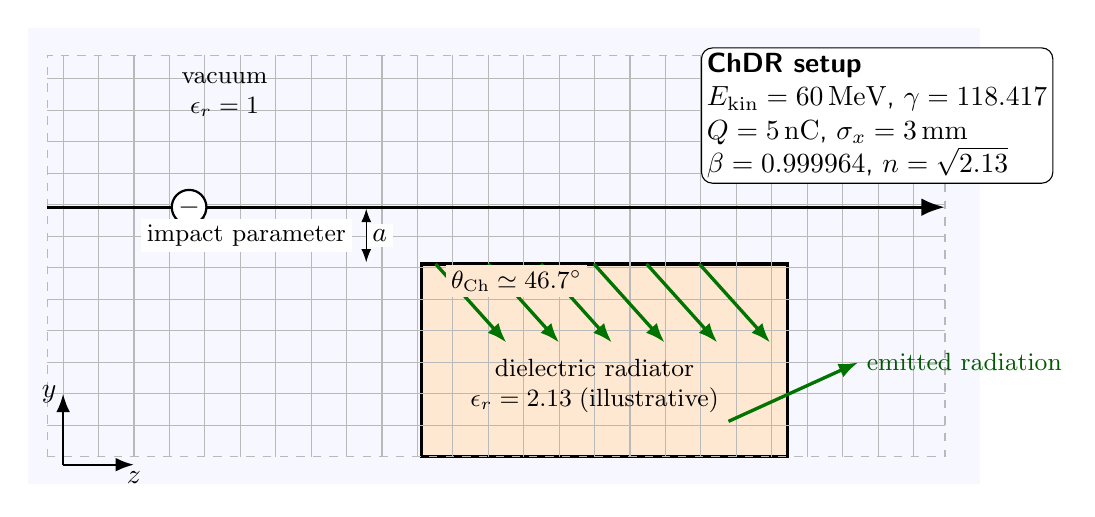
\begin{tikzpicture}[
  x=1cm,
  z=1cm,
  >=Latex,
  font=\sffamily,
  beam/.style={very thick, -{Latex[length=3mm]}},
  radiation/.style={very thick, -{Latex[length=2.5mm]}, green!45!black},
  boundary/.style={very thick, black},
  gridline/.style={thin, gray!55},
  label/.style={font=\small},
  every node/.style={inner sep=2pt}
]

  % Vacuum background and dielectric radiator.
  \fill[blue!3] (-1.0,-2.8) rectangle (11.1,3.0);
  \fill[orange!18] (4.0,-2.45) rectangle (8.65,0.0);
  \draw[boundary] (4.0,0.0) -- (8.65,0.0) -- (8.65,-2.45)
                  -- (4.0,-2.45) -- cycle;

  % Computational mesh spanning both vacuum and dielectric.
  \foreach \xx in {-0.55,-0.10,0.35,0.80,1.25,1.70,2.15,2.60,3.05,3.50,
                    3.95,4.40,4.85,5.30,5.75,6.20,6.65,7.10,7.55,8.00,
                    8.45,8.90,9.35,9.80,10.25}
    \draw[gridline] (\xx,-2.45) -- (\xx,2.65);
  \foreach \yy in {-2.05,-1.65,-1.25,-0.85,-0.45,-0.05,0.35,0.75,
                    1.15,1.55,1.95,2.35}
    \draw[gridline] (-0.75,\yy) -- (10.65,\yy);
  \draw[gridline,dashed] (-0.75,-2.45) rectangle (10.65,2.65);

  % Beam travelling in +x, parallel to the dielectric surface.
  \draw[beam] (-0.75,0.72) -- (10.65,0.72);

  % A small bunch marker and negative charge sign.
  \draw[thick,fill=white] (1.05,0.72) circle (0.22);
  \node at (1.05,0.72) {$-$};

  % Beam--surface impact parameter.
  \draw[<->] (3.30,0.02) -- node[right,fill=white] {$a$} (3.30,0.70);
  \node[label,anchor=east,fill=white] at (3.12,0.36) {impact parameter};

  % Radiation generated in the dielectric at the Cherenkov angle.
  \draw[radiation] (4.18,0.0) -- (5.08,-1.00);
  \draw[radiation] (4.85,0.0) -- (5.75,-1.00);
  \draw[radiation] (5.52,0.0) -- (6.42,-1.00);
  \draw[radiation] (6.19,0.0) -- (7.09,-1.00);
  \draw[radiation] (6.86,0.0) -- (7.76,-1.00);
  \draw[radiation] (7.53,0.0) -- (8.43,-1.00);

  % One representative ray exiting the finite radiator.
  \draw[radiation] (7.90,-2.00) -- (9.55,-1.25);
  \node[label,anchor=west,green!35!black] at (9.58,-1.25)
    {emitted radiation};

  % Cherenkov angle, measured from the beam direction (+x).
  \draw[thin] (4.18,0.0) ++(-48:0.55)
    arc[start angle=-48,end angle=0,radius=0.55];
  \node[label,anchor=west,fill=orange!18] at (4.30,-0.22)
    {$\theta_{\rm Ch}\simeq46.7^\circ$};

  % Material labels.
  \node[label,align=center] at (6.20,-1.55)
    {dielectric radiator\\
     $\epsilon_r=2.13$\;(illustrative)};
  \node[label,align=center] at (1.50,2.15)
    {vacuum\\$\epsilon_r=1$};

  % Coordinate axes.
  \draw[->,thick] (-0.55,-2.55) -- (-0.55,-1.65)
    node[left] {$y$};
  \draw[->,thick] (-0.55,-2.55) -- (0.35,-2.55)
    node[below] {$z$};

  % A compact parameter box.
  \node[draw,rounded corners,fill=white,align=left,anchor=north west]
    at (7.55,2.75) {\textbf{ChDR setup}\\
      $E_{\rm kin}=60\,\si{MeV}$, $\gamma=118.417$\\
      $Q=5\,\si{nC}$, $\sigma_x=3\,\si{mm}$\\
      $\beta=0.999964$, $n=\sqrt{2.13}$};

\end{tikzpicture}

\caption{Schematic $x$--$z$ view of the Cherenkov-diffraction-radiation setup.  The continuous grid represents the computational domain in both vacuum and dielectric.}
\end{figure}

\end{document}
